\begin{frame}[fragile,label=OAresults,shrink=5]{The structure of the interval $[\beta^*, \hbeta]\leq \bCon \bA$.}

\vskip2mm

  \begin{itemize}
  \item If $\beta \in \Con \bB$ is a coatom of $\bCon \bB$ with $m$ congruence classes then
        the interval $[\beta^*, \hbeta]$ in $\bCon \bA$ is $\two^{m-1}$.
  \end{itemize}

  \begin{columns}
    \begin{column}{0.3\textwidth}

      {\scalefont{.8}
        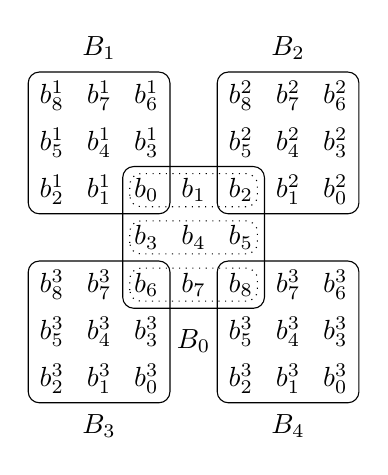
\begin{tikzpicture}[scale=.6]
          \draw[rounded corners] (-1.5,-1.5) rectangle (1.5,1.5);
          \draw[rounded corners] (.5,.5) rectangle (3.5,3.5);
          \visible<2->{\draw[rounded corners] (.5,-3.5) rectangle (3.5,-.5) (-3.5,-3.5) rectangle (-.5,-.5);}
          \draw[rounded corners] (-3.5,.5) rectangle (-.5,3.5);
          \draw[rounded corners, dotted] (-1.35,.65) rectangle (1.35,1.35);  
          \draw[rounded corners, dotted] (-1.35,-.35) rectangle (1.35,.35);
          \draw[rounded corners, dotted] (-1.35,-1.35) rectangle (1.35,-.65);

          \draw (0,-2.2) node {$B_0 $};
          %%    % B1
          \draw (-2, 4) node {$B_1$};
          \draw (-1, 1) node {$b_0$};
          \foreach \i in {0,1,2} {
            \foreach \j in {1,2} {
              \pgfmathtruncatemacro{\x}{3*\i+\j}
              \draw (-\j - 1, \i + 1) node {$b^1_\x$};
            }
          }
          \foreach \i in {1,2} {
            \foreach \j in {0} {
              \pgfmathtruncatemacro{\x}{3*\i+\j}
              \draw (-\j - 1, \i + 1) node {$b^1_\x$};
            }
          }
          \draw (0, 1) node {$b_1$};

          %%    % B2
          \draw (2, 4) node {$B_2$};
          \draw (1, 1) node {$b_2$};
          \foreach \i in {0,1,2} {
            \foreach \j in {1,2} {
              \pgfmathtruncatemacro{\x}{3*\i+(2-\j)}
              \draw (\j + 1, \i + 1) node {$b^2_\x$};
            }
          }
          \foreach \i in {1,2} {
            \foreach \j in {0} {
              \pgfmathtruncatemacro{\x}{3*\i+(2-\j)}
              \draw (\j + 1, \i + 1) node {$b^2_\x$};
            }
          }
          \foreach \j in {3,4,5} {
            \draw (\j -4, 0) node {$b_\j$};
          }

          \foreach \j in {6,7,8} {
            \draw (\j -7, -1) node {$b_\j$};
          }
          \visible<2->{
            %%    % B3
            \draw (-2, -4) node {$B_3$};

            \foreach \i in {0,1,2} {
              \foreach \j in {1,2} {
                \pgfmathtruncatemacro{\x}{3*(2-\i)+\j}
                \draw (-\j - 1, -\i - 1) node {$b^3_\x$};
              }
            }
            \foreach \i in {1,2} {
              \foreach \j in {0} {
                \pgfmathtruncatemacro{\x}{3*(2-\i)+\j}
                \draw (-\j - 1, -\i - 1) node {$b^3_\x$};
              }
            }

            %%    % B4
            \draw (2, -4) node {$B_4$};
            \foreach \i in {1,2} {
              \foreach \j in {0,1,2} {
                \pgfmathtruncatemacro{\x}{3*(2-\i)+\j}
                \draw (3-\j , -\i - 1) node {$b^3_\x$};
              }
            }
            \foreach \i in {0} {
              \foreach \j in {0,1} {
                \pgfmathtruncatemacro{\x}{3*(2-\i)+\j}
                \draw (3-\j, -\i - 1) node {$b^3_\x$};
              }
            }
          }
        \end{tikzpicture}
      }
    \end{column}
    \begin{column}{0.6\textwidth}
      \vskip2mm
      \uncover<2->{
        \emph{More generally...}
        \vskip4pt
        \begin{itemize}
        \item  Suppose $\beta \in \Con \bB$ has transversal $b_{\beta(1)}, \dots, b_{\beta(m)}$.
          \vskip10pt
        \item Denote by $T_r$ the set of intersection points in the $r$-th block of $\beta$:
          \[
          T_r
          =  \bigcup_{k=1}^K B_k \cap b_{\beta(r)}/\beta.
          \]
        \end{itemize}
      }
    \end{column}
  \end{columns}
  %% \begin{columns}
  %%   \begin{column}{0.7\textwidth}
      \visible<3->{
        %        \begin{theorem}
        \vskip-2mm
        \begin{block}{}{}
          \[   \text{Then} \quad       [\beta^*, \widehat{\beta}] 
          = 
          \{\theta \in \Eq(A) : \beta^* \subseteq \theta \subseteq \widehat{\beta} \}
          \cong \prod_{r=1}^m (\Eq |T_r|)^{m-1}.
          \]
        \end{block}
      }

  %%   \end{column}
  %% \end{columns}
\end{frame}

\begin{frame}[fragile,label=OAextension,shrink=5]{Slightly more general examples...}

  Returning to our original example, the base algebra $\bB$
  is the right regular $S_3$-set, and the nontrivial relations in $\Con \bB$ are
  \vskip-2pt
  %% \begin{align*}
  %%   \alpha &=  \pb 0, 1, 2 \pb 3, 4, 5\pb \\[4pt]
  %%   \beta &=  \pb 0, 3 \pb 1, 4 \pb 2, 5 \pb \\[3pt]
  %%   \gamma &= |0, 4| 1, 5|2, 3| \\[3pt]
  %%   \delta &= |0, 5|1, 3|2, 4| 
  %% \end{align*}
\[
    \alpha =  \pb 0, 1, 2 \pb 3, 4, 5\pb \quad
    \beta =  \pb 0, 3 \pb 1, 4 \pb 2, 5 \pb \quad
    \gamma = |0, 4| 1, 5|2, 3| \quad
    \delta = |0, 5|1, 3|2, 4| \]

    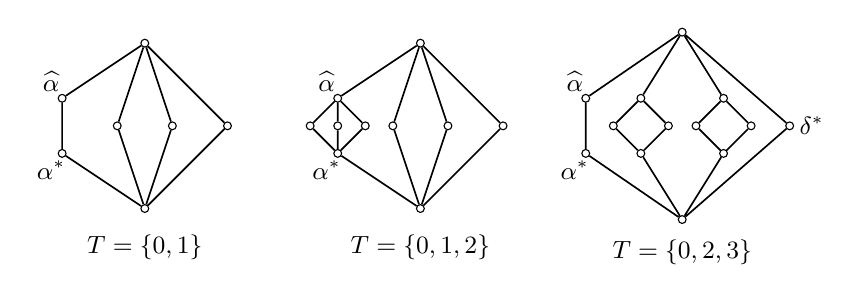
\begin{tikzpicture}[scale=.7]
      % T = \{0, 1\}
      \node (150) at (1.5,0)  [draw, circle, inner sep=1.0pt] {};
      \node (01) at (0,1)  [draw, circle, inner sep=1.0pt] {};
      \node (02) at (0,2)  [draw, circle, inner sep=1.0pt] {};
      \node (115) at (1,1.5)  [draw, circle, inner sep=1.0pt] {};
      \node (215) at (2,1.5)  [draw, circle, inner sep=1.0pt] {};
      \node (315) at (3,1.5)  [draw, circle, inner sep=1.0pt] {};
      \node (153) at (1.5,3)  [draw, circle, inner sep=1.0pt] {};
      \draw[semithick] 
      (150) to (01) to (02) to (153) to (115) to (150) to (215) to (153) to (315) to (150);
      \draw[font=\small] (1.5,-.7) node {$T = \{0,1\}$};
      \draw[font=\small] (-.2,.7) node {$\alpha^*$};
      \draw[font=\small] (-.2,2.3) node {$\widehat{\alpha}$};

      % T = \{0, 1, 2\}
      \node (650) at (6.5,0)  [draw, circle, inner sep=1.0pt] {};
      \node (51) at (5,1)  [draw, circle, inner sep=1.0pt] {};
      \node (52) at (5,2)  [draw, circle, inner sep=1.0pt] {};
      \node (4515) at (4.5,1.5)  [draw, circle, inner sep=1.0pt] {};
      \node (515) at (5,1.5)  [draw, circle, inner sep=1.0pt] {};
      \node (5515) at (5.5,1.5)  [draw, circle, inner sep=1.0pt] {};
      \node (615) at (6,1.5)  [draw, circle, inner sep=1.0pt] {};
      \node (715) at (7,1.5)  [draw, circle, inner sep=1.0pt] {};
      \node (815) at (8,1.5)  [draw, circle, inner sep=1.0pt] {};
      \node (653) at (6.5,3)  [draw, circle, inner sep=1.0pt] {};
      \draw[semithick] 
      (650) to (51) to (515) to (52) to (653) to (615) to (650) to (715) to (653) to
      (815) to (650)
      (51) to (4515) to (52) to (5515) to (51);
      \draw[font=\small] (6.5,-.7) node {$T = \{0,1,2\}$};
      \draw[font=\small] (4.8,.7) node {$\alpha^*$};
      \draw[font=\small] (4.8,2.3) node {$\widehat{\alpha}$};

      % T = \{0, 2, 3\}
      \node (bot) at (11.25,-.2)  [draw, circle, inner sep=1.0pt] {};
      \node (top) at (11.25,3.2)  [draw, circle, inner sep=1.0pt] {};
      \node (a) at (9.5,1)  [draw, circle, inner sep=1.0pt] {};
      \node (A) at (9.5,2)  [draw, circle, inner sep=1.0pt] {};
      \draw[font=\small] (9.3,.7) node {$\alpha^*$};
      \draw[font=\small] (9.3,2.3) node {$\widehat{\alpha}$};


      \node (b) at (10.5,1)  [draw, circle, inner sep=1.0pt] {};
      \node (b1) at (10,1.5)  [draw, circle, inner sep=1.0pt] {};
      \node (b2) at (11,1.5)  [draw, circle, inner sep=1.0pt] {};
      \node (B) at (10.5,2)  [draw, circle, inner sep=1.0pt] {};

      \node (c) at (12,1)  [draw, circle, inner sep=1.0pt] {};
      \node (c1) at (11.5,1.5)  [draw, circle, inner sep=1.0pt] {};
      \node (c2) at (12.5,1.5)  [draw, circle, inner sep=1.0pt] {};
      \node (C) at (12,2)  [draw, circle, inner sep=1.0pt] {};

      \node (d) at (13.2,1.5)  [draw, circle, inner sep=1.0pt] {};
      \draw[font=\small] (13.6,1.5) node {$\delta^*$};
      \draw[semithick] 
      (bot) to (a) to (A) to (top) to (B) to (b1) to (b) to (b2) to (B)
      (b) to (bot) to (c) to (c1) to (C) to (c2) to (c)
      (C) to (top) to (d) to (bot);
      \draw[font=\small] (11.25,-.8) node {$T = \{0, 2, 3\}$};

    \end{tikzpicture}

    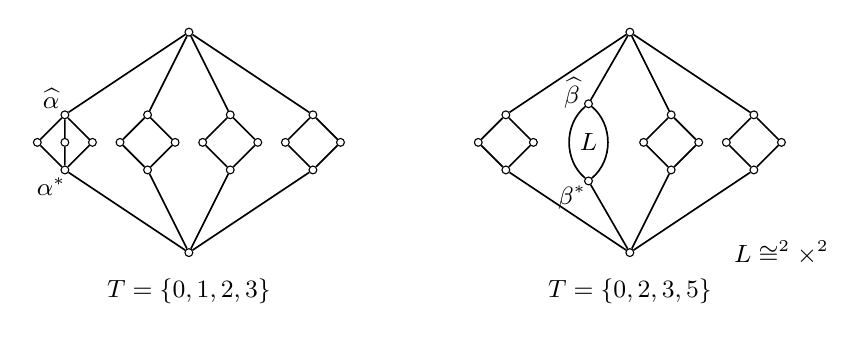
\begin{tikzpicture}[scale=.7]
      % T = \{0, 1, 2, 3\}
      \node (bot) at (3.25,0.5)  [draw, circle, inner sep=1.0pt] {};
      \node (top) at (3.25,4.5)  [draw, circle, inner sep=1.0pt] {};

      \node (a) at (1,2)  [draw, circle, inner sep=1.0pt] {};
      \node (a1) at (.5,2.5)  [draw, circle, inner sep=1.0pt] {};
      \node (a2) at (1,2.5)  [draw, circle, inner sep=1.0pt] {};
      \node (a3) at (1.5,2.5)  [draw, circle, inner sep=1.0pt] {};
      \node (A) at (1,3)  [draw, circle, inner sep=1.0pt] {};
      \draw[font=\small] (.75,1.7) node {$\alpha^*$};
      \draw[font=\small] (.75,3.3) node {$\widehat{\alpha}$};

      \node (b) at (2.5,2)  [draw, circle, inner sep=1.0pt] {};
      \node (b1) at (2,2.5)  [draw, circle, inner sep=1.0pt] {};
      \node (b2) at (3,2.5)  [draw, circle, inner sep=1.0pt] {};
      \node (B) at (2.5,3)  [draw, circle, inner sep=1.0pt] {};

      \node (c) at (4,2)  [draw, circle, inner sep=1.0pt] {};
      \node (c1) at (3.5,2.5)  [draw, circle, inner sep=1.0pt] {};
      \node (c2) at (4.5,2.5)  [draw, circle, inner sep=1.0pt] {};
      \node (C) at (4,3)  [draw, circle, inner sep=1.0pt] {};

      \node (d) at (5.5,2)  [draw, circle, inner sep=1.0pt] {};
      \node (d1) at (5,2.5)  [draw, circle, inner sep=1.0pt] {};
      \node (d2) at (6,2.5)  [draw, circle, inner sep=1.0pt] {};
      \node (D) at (5.5,3)  [draw, circle, inner sep=1.0pt] {};

      \draw[semithick] 
      (bot) to (a) to (a1) to (A) to (a2) to (a) to (a3) to (A) to (top) to 
      (B) to (b1) to (b) to (b2) to (B)
      (b) to (bot) to (c) to (c1) to (C) to (c2) to (c)
      (C) to (top) to (D) to (d1) to (d) to (d2) to (D)
      (d) to (bot);
      \draw[font=\small] (3.25,-.2) node {$T = \{0,1,2,3\}$};

      % T = \{0, 2, 3, 5\}
      \node (Rbot) at (11.25,0.5)  [draw, circle, inner sep=1.0pt] {};
      \node (Rtop) at (11.25,4.5)  [draw, circle, inner sep=1.0pt] {};

      \node (Ra) at (9,2)  [draw, circle, inner sep=1.0pt] {};
      \node (Ra1) at (8.5,2.5)  [draw, circle, inner sep=1.0pt] {};
      \node (Ra2) at (9.5,2.5)  [draw, circle, inner sep=1.0pt] {};
      \node (RA) at (9,3)  [draw, circle, inner sep=1.0pt] {};

      \node (Rb) at (10.5,1.8)  [draw, circle, inner sep=1.0pt] {};
      \node (RB) at (10.5,3.2)  [draw, circle, inner sep=1.0pt] {};
      \draw[font=\small] (10.2,1.5) node {$\beta^*$};
      \draw[font=\small] (10.2,3.4) node {$\widehat{\beta}$};

      \node (Rc) at (12,2)  [draw, circle, inner sep=1.0pt] {};
      \node (Rc1) at (11.5,2.5)  [draw, circle, inner sep=1.0pt] {};
      \node (Rc2) at (12.5,2.5)  [draw, circle, inner sep=1.0pt] {};
      \node (RC) at (12,3)  [draw, circle, inner sep=1.0pt] {};

      \node (Rd) at (13.5,2)  [draw, circle, inner sep=1.0pt] {};
      \node (Rd1) at (13,2.5)  [draw, circle, inner sep=1.0pt] {};
      \node (Rd2) at (14,2.5)  [draw, circle, inner sep=1.0pt] {};
      \node (RD) at (13.5,3)  [draw, circle, inner sep=1.0pt] {};

      \draw[semithick] 
      (Rbot) to (Ra) to (Ra1) to (RA) to (Ra2) to (Ra) 
      (RA) to (Rtop) to (RB)
      (Rb) to (Rbot) to (Rc) to (Rc1) to (RC) to (Rc2) to (Rc)
      (RC) to (Rtop) to (RD) to (Rd1) to (Rd) to (Rd2) to (RD)
      (Rd) to (Rbot);
      \draw [semithick]  
      (Rb) to [out=140,in=-140] (RB)
      (RB) to [out=-40,in=40] (Rb);
      \draw[font=\small] (10.5,2.5) node {$L$};

      \draw[font=\small] (11.25,-.2) node {$T = \{0,2,3, 5\}$};
      \draw[font=\small] (14,.5) node {$L\cong \two^2\times\two^2$};

    \end{tikzpicture}
\end{frame}
%% Since $\beta = | 0, 3 | 2, 5 | 1, 4 |$, when $T = \{0,2,3, 5\}$, the interval
%% $[\beta^*,\widehat{\beta}]$ is 
%% %$\Eq(2)^2 \times \Eq(2)^2  = \two^2\times\two^2$.  
%% $\two^2\times\two^2$.  
%% In Figure~\ref{fig:ConOverAlgebras2}, we denote this abstractly by $L$,
%% instead of drawing all 16 points of this interval.

%% \end{example}

%% Next, consider the situation depicted in the last congruence lattice of
%% Figure~\ref{fig:ConOverAlgebras2}, where 
%% $L \cong \two^2\times\two^2$, and
%% suppose we prefer that all the other $\resB$-inverse images be trivial:
%% $
%% [\beta^*,\widehat{\beta}]\cong \two^2\times\two^2; \,%\quad 
%% \alpha^*=\widehat{\alpha}; \, %\quad
%% \gamma^*=\widehat{\gamma};\,  %\quad
%% \delta^*=\widehat{\delta}.
%% $
%% In other words, we seek a finite algebraic
%% representation of the lattice in Figure~\ref{fig:ConOverAlgebras3}.
%% \begin{figure}[h!]
%%   \centering
%%     \begin{tikzpicture}[scale=.6]
%%       \node (Rbot) at (11.25,0.5)  [draw, circle, inner sep=1.0pt] {};
%%       \node (Rtop) at (11.25,4.5)  [draw, circle, inner sep=1.0pt] {};
%%       \node (Ra) at (9.25,2.5)  [draw, circle, inner sep=1.0pt] {};
%%       \node (Rb) at (10.75,1.8)  [draw, circle, inner sep=1.0pt] {};
%%       \node (RB) at (10.75,3.2)  [draw, circle, inner sep=1.0pt] {};
%%       \node (Rc) at (12,2.5)  [draw, circle, inner sep=1.0pt] {};
%%       \node (Rd) at (13.25,2.5)  [draw, circle, inner sep=1.0pt] {};
%%       \draw[semithick] 
%%       (Rbot) to (Ra) to (Rtop) to (RB)
%%       (Rb) to (Rbot) to (Rc) to (Rtop) to (Rd) to (Rbot);
%%       \draw [semithick]  
%%       (Rb) to [out=140,in=-140] (RB)
%%       (RB) to [out=-40,in=40] (Rb);
%%       \draw[font=\small] (10.75,2.5) node {$L$};
%%     \end{tikzpicture}
%%   \caption{A lattice which motivates further expansion of the set of basic 
%%     operations in the overalgebra.}
%%   \label{fig:ConOverAlgebras3}
%% \end{figure}
%% This is easy to achieve by adding more operations in the overalgebra
%% construction described above.
%% In fact, it is possible to introduce additional operations
%% so that, if $\beta = \Cg^\bB(x,y)$, then $\theta^* = \widehat{\theta}$ for all
%% $\theta \in \Con\bB$ with $\theta \ngeq \beta$. %%   \begin{itemize}
%%   \item put stuff here...
%%   \end{itemize}
%% \end{frame}

%% \begin{frame}[fragile,label=Extensions,shrink=5]{Generalizations...}
%%   \begin{itemize}
%%   \item put stuff here...
%%   \end{itemize}
%% \end{frame}

\begin{frame}[fragile,label=Limitations,shrink=5]{Limitations}

\vskip5mm

Two limitations of the foregoing construction:
\begin{enumerate}
\item The sizes $|T_r|$ of the partition lattice factors in 
\[
[\beta^*, \widehat{\beta}] \cong \prod_{r=1}^m (\Eq |T_r|)^{m-1}
\] 
are limited by the size of the blocks of $\beta$.

\vskip3mm

\item If $\beta$ is not principal, 
$[\theta^*, \htheta]$ may be non-trivial for some $\theta \ngeq \beta$.
\end{enumerate}
\end{frame}

\begin{frame}[fragile,label=OAextension2,shrink=5]{A Generalization}
 %% \begin{columns}
 %%  \begin{column}{0.8\textwidth}

\begin{theorem}
Let $\bB = \<B, F\>$ be a finite algebra. Suppose
\[
\beta = \Cg^{\bB}((a_1, b_1), \dots, (a_{K-1},b_{K-1}))
\]
has $m$ blocks and fix $N<\infty$.

\vskip3mm

There exists an overalgebra $\<A, F_A\>$
%Then, $\beta^* = \Cg^{\bA}(\beta)$ is given by
such that the interval $\beta\resB^{-1} \leq \Con \bA$ is 
%If $\beta$ has transversal $\{a_1, c_1, c_2, \dots, c_{m-1}\}$, then
%{\small \[ 
%% \beta^* = \bigcup_{j=0}^{MK} \beta^{\bB_j} \cup 
%% \left(\bigcup_{i=0}^{MK}t_i/\beta^{\bB_i}\right)^2, \quad
%%   \widehat{\beta} = \beta^* 
%% \cup 
%% \bigcup_{i=1}^{m-1}\left(\bigcup_{\ell \in \sE} c_i^\ell/\beta^{\bB_{\ell}}\right)^2
%% \cup 
%% \bigcup_{i=1}^{m-1}\left(\bigcup_{\ell \in \sO}
%% c_i^\ell/\beta^{\bB_{\ell}}\right)^2.
%% \]}
\[
[\beta^*, \widehat{\beta}] \cong (\Eq (N))^{m-1}.
\]
Moreover, we can arrange it so that $\theta^* = \widehat{\theta}$ for all $\theta \ngeq \beta$ in $\Con \bA$.
\end{theorem}

  %% \end{column}
  %% \begin{column}{0.2\textwidth}

%% \begin{align*}
%% B_0\cap B_1 &=\{a_1\}=\{a_1^{1}\},\\
%% B_1\cap B_2 &=\{b^1_1\}=\{a_2^{2}\},\\
%% B_2\cap B_3 &=\{b^2_2\}=\{a_3^{3}\},\\
%% \vdots\\
%% B_{K-2}\cap B_{K-1} &= \{b_{K-2}^{K-2}\}=\{a_{K-1}^{K-1}\},\\
%% B_{K-1}\cap B_K = B_K\cap B_{K+1}&=\{b^{K-1}_{K-1}\}=\{b^{K}_{K-1}\}=\{b^{K+1}_{K-1}\},\\
%% B_{K+1}\cap B_{K+2}&=\{a^{K+1}_{K-1}\} =\{b^{K+2}_{K-2}\},\\
%% B_{K+2}\cap B_{K+3}&=\{a^{K+2}_{K-2}\} =\{b^{K+3}_{K-3}\},\\
%% \vdots\\
%% B_{2K-2}\cap B_{2K-1} &= \{a_{2}^{2K-2}\}=\{b_{1}^{2K-1}\},\\
%% B_{2K-1}\cap B_{2K} = B_{2K}\cap  B_{2K+1}&=\{a^{2K-1}_{1}\}=\{a^{2K}_{1}\}=\{a^{2K+1}_{1}\},\\
%% B_{2K+1}\cap B_{2K+2}&=\{b^{2K+1}_{1}\} =\{b^{2K+2}_{2}\},\\
%% B_{2K+2}\cap B_{2K+3}&=\{b^{2K+2}_{2}\} =\{b^{2K+3}_{3}\},\\
%% \vdots\\
%% B_{MK-2}\cap B_{MK-1} &= \{b_{MK-2}^{K-2}\}=\{a_{MK-1}^{K-1}\},\\
%% B_{MK-1}\cap B_{MK}&=\{b^{MK-1}_{K-1}\}=\{b^{MK}_{K-1}\}.
%% \end{align*}
%% All other intersections are empty.
%%   \end{column}
%%  \end{columns}

\vskip3mm
\uncover<2->{
{\scalefont{.7}
  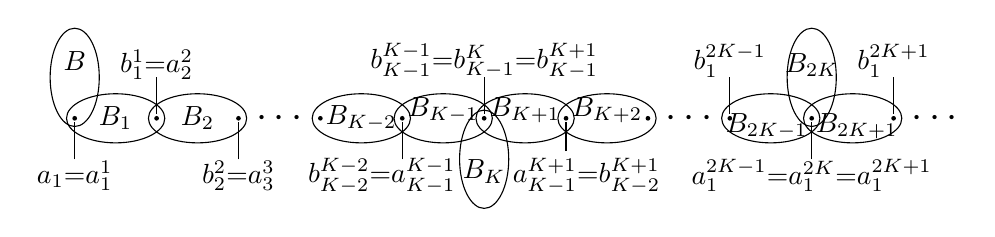
\begin{tikzpicture}[scale=.52]
    % B0
    \draw (0, 3.4) node {$B$};
    \draw (0,3) ellipse (.6cm and 1.2cm);

    % B1
    \draw (1,2) node {$B_1$};
    \draw (1,2) ellipse (1.2cm and .6cm);

    % B2
    \draw (3,2) node {$B_2$};
    \draw (3,2) ellipse (1.2cm and .6cm);

   \draw[font=\Large] (5, 2) node {$\cdots$};

    \draw (7,2) node {$B_{K-2}$};
    \draw (7,2) ellipse (1.2cm and .6cm);

    \draw (9,2.2) node {$B_{K-1}$};
    \draw (9,2) ellipse (1.2cm and .6cm);

    \draw (10,.7) node {$B_{K}$};
    \draw (10,1) ellipse (.6cm and 1.2cm);

    \draw (11,2.2) node {$B_{K+1}$};
    \draw (11,2) ellipse (1.2cm and .6cm);

    \draw (13,2.2) node {$B_{K+2}$};
    \draw (13,2) ellipse (1.2cm and .6cm);


   \draw[font=\Large] (15, 2) node {$\cdots$};

    \draw (16.9,1.8) node {$B_{2K-1}$};
    \draw (17,2) ellipse (1.2cm and .6cm);

    \draw (18,3.3) node {$B_{2K}$};
    \draw (18,3) ellipse (.6cm and 1.2cm);

    \draw (19.1,1.8) node {$B_{2K+1}$};
    \draw (19,2) ellipse (1.2cm and .6cm);

   \draw[font=\Large] (21, 2) node {$\cdots$};

   \node (1) at (0,2) [fill,circle,inner sep=.6pt] {};
   \draw (0, .6) node {$a_1{=}a_1^1$};
   \draw (0, 1) to  (0,1.9);

   \node (2) at (2,2) [fill,circle,inner sep=.6pt] {};
   \draw (2, 3.3) node {$b^1_1 {=} a^2_2$};
   \draw (2, 3) to  (2,2.1);

   \node (3) at (4,2) [fill,circle,inner sep=.6pt] {};
   \draw (4, .6) node {$b^2_2 {=} a^3_3$};
   \draw (4, 1) to  (4,1.9);

   \node (4) at (6,2) [fill,circle,inner sep=.6pt] {};
   \node (5) at (8,2) [fill,circle,inner sep=.6pt] {};
  \draw (7.5, .6) node {$b^{K-2}_{K-2} {=} a^{K-1}_{K-1}$};
   \draw (8, 1) to  (8,1.9);

   \node (6) at (10,2) [fill,circle,inner sep=.6pt] {};
   \draw (10, 3.4) node {$b^{K-1}_{K-1} {=} b^{K}_{K-1}{=} b^{K+1}_{K-1}$};
   \draw (10, 3) to  (10,2.1);

   \node (7) at (12,2) [fill,circle,inner sep=.6pt] {};
   \draw (12.5, .6) node {$a^{K+1}_{K-1} {=} b^{K+1}_{K-2}$};
   \draw (12, 1.2) to  (12,1.9);

   \node (8) at (14,2) [fill,circle,inner sep=.6pt] {};

   \node (9) at (16,2) [fill,circle,inner sep=.6pt] {};
   \draw (16, 3.4) node {$b^{2K-1}_{1}$};
   \draw (16, 3) to  (16,2.1);

   \node (10) at (18,2) [fill,circle,inner sep=.6pt] {};
   \draw (18, .6) node {$a^{2K-1}_{1} {=} a^{2K}_{1}{=} a^{2K+1}_{1}$};
   \draw (18, 1) to  (18,1.9);

   \node (11) at (20,2) [fill,circle,inner sep=.6pt] {};
   \draw (20, 3.4) node {$b^{2K+1}_{1}$};
   \draw (20, 3) to  (20,2.1);
   
  \end{tikzpicture}
}
}
\end{frame}

